\documentclass[a4paper]{report}
\usepackage{amsmath, amssymb}
\usepackage{float}
\usepackage{graphicx}
\usepackage{xcolor}
\usepackage{algorithm}
\usepackage{algpseudocode}
\usepackage{caption}
\usepackage{subcaption} % For subfigures
\usepackage{setspace} % For line spacing
\usepackage{booktabs} % For formal tables
\usepackage{microtype} % For better typesetting (dense text etc.)
\usepackage{tikz}
\usepackage{hyperref} % For hyperlinks
\usepackage{listings} % For code snippets
\usepackage{longtable} % For long tables
\usepackage[acronym]{glossaries} % For glossaries
\usepackage[margin=1in]{geometry} % For page margins
\usepackage{eso-pic} % Needed for AddToShipoutPicture
\usetikzlibrary{calc}
\usepackage[
backend=biber,
style=authoryear-icomp,
sorting=ynt
]{biblatex}
\addbibresource{kiva-writing.bib}
\setstretch{1.25}

\newcommand{\todo}[1]{\textcolor{red}{TODO: #1}}
\newcommand{\note}[1]{\textcolor{blue}{NOTE: #1}}
\newcommand{\densetext}[1]{\scalebox{0.8}[1.0]{\textls[-80]{#1}}}
\DeclareMathOperator*{\argmax}{argmax} % no space, limits underneath in displays

\makeglossaries
\newacronym{cf}{CF}{Crowdfunding}
\newacronym{cfp}{CFPs}{Crowdfunding Platforms}

\newglossaryentry{activity}{
	name=activity,
	description={A property of loan which is more descriptive than Sector}
}

\newglossaryentry{sector}{
	name=sector,
	description={A sector is a broad category for a loan, e.g. Agriculture, Arts, Clothing. Sectors are subdivided further by activities.}
}

\newglossaryentry{tag}{
	name=tag,
	description={Loan properties which are attributed by lenders}
}




\begin{document}

% Draw a border on every page
\AddToShipoutPicture{%
	\begin{tikzpicture}[overlay,remember picture]
		\draw [line width=1pt]
		($ (current page.north west) + (0.5cm,-0.5cm) $) rectangle
		($ (current page.south east) + (-0.5cm,0.5cm) $);
	\end{tikzpicture}%
}

% checked with https://capitalizemytitle.com/style/APA/
\title{Detecting Community Dynamics on Crowdfunding Platforms}
\author{Tien-Dat NGUYEN}
\date{Dec 2023}
% \maketitle

\begin{titlepage}
	\centering
	\vspace*{1cm}

	% University Name
	{\Large \textbf{UNIVERSITY OF PARIS-SACLAY, VNU UNIVERSITY OF ENGINEERING AND TECHNOLOGY}}\\[1cm]

	
\includegraphics[width=0.7\textwidth]{images/logo_combine.png}
	\vspace*{4cm}


	% Subject Name
	{\Large \textbf{MASTER'S THESIS}}\\[0.5cm]

	% Report Name
	{\Huge \textbf{DETECTING COMMUNITY DYNAMICS ON CROWDFUNDING PLATFORMS} \par}
	\vspace*{2cm}
	% Advisor's Name
	{\large \textbf{Advisors:}}
	\begin{large}
		\begin{itemize}
			\item Prof. Natacha CHETCUTI-OSOROVITZ
			\item Prof. Salah EL AYOUBI
			\item Prof. TRAN Trong Hieu
		\end{itemize}
	\end{large}
	\vspace*{1cm}
	% Student's Name
	{\large \textbf{Student:} Tien-Dat NGUYEN}\\[0.5cm]

	{\large \textbf{Internship location:} Laboratoire des Signaux et Systèmes, L2S - CentraleSupélec - Université Paris-Saclay}\\[0.25cm]

	% Location and Date
	{\large GIF-SUR-YVETTE, Dec 2023 }\\[0.25cm]


	% Fill the rest of the page with whitespace
	\vfill
\end{titlepage}
\tableofcontents
\listoffigures
\listoftables

% \clearpage
\printglossary
\printglossary[type=\acronymtype]

\chapter{Introduction}
\begin{comment}
Content should be contain in this chapter

\begin{itemize}
	\item The dynamic of crowdfunding is rather complex and not well-understood
	\item We would like to understand the role of community in crowdfunding
	      \begin{itemize}
		      \item Hypothesis: there might be communities (explicit or implicit) of lenders (contributors) who willing to contribute to same type of projects again and again
		            \begin{itemize}
			            \item Describe the hypothesis in more details. What is type of projects?
		            \end{itemize}
	      \end{itemize}
	\item The objective of the thesis is to Detect Community Dynamic. If it exists on platforms?
	\item We will test the hypothesis on kiva.org dataset
	\item \textit{Briefly} describe the kiva platform
	      \begin{itemize}
		      \item What is kiva.org and how it works?
		      \item Overview of the data schema: Lender, Project, Sector, Tags, and how those can be viewed as a graph
		      \item What is type of projects in this dataset?
		            \begin{itemize}
			            \item Type means \textit{type of impact} or \textit{localization}
			                  \begin{itemize}
				                  \item Type of impact: impact more on sociality, impact more on environments,... Represented by Sector or Tags
				                  \item Localization: represent by country where borrower live in
			                  \end{itemize}
		            \end{itemize}
	      \end{itemize}
	\item \textit{Briefly} describe how we will work:
	      \begin{itemize}
		      \item Given the graph-like database, we will find community of lenders in the database using \textit{community finding on graphs} techniques
		      \item This is a unsupervised problem
	      \end{itemize}
\end{itemize}
\end{comment}

Crowdfunding has become an increasingly popular way for entrepreneurs and innovators to raise funds for their projects.
It is a process of raising small amounts of money from a large number of people, typically via the Internet.
Researchers have studied crowdfunding from different perspectives, such as the impact of crowdfunding on the economy, or the role of social networks.
The success of crowdfunding campaigns, however, is rather complex and still not well-understood.
Through qualitative research, scholars believe that community is a factor that influences the success of crowdfunding campaigns.
In this thesis, we study the role of community in crowdfunding quantitatively via data analysis.

We hypothesize that there might be communities (explicit or implicit) of lenders (contributors) who are willing to contribute to the same type of projects again and again.
The objective of this thesis is to detect the existing of such communities on crowdfunding platforms.

We will test this hypothesis on the Kiva.org platform,
which is a crowdfunding platform that allows people to lend money to low-income entrepreneurs and students in over 80 countries.
Through API, we will collect data about Lenders, Projects, Sectors, Tags, Countries and the relationships between them.
We then build a graph-like database from the collected data,
and apply community detection on graphs techniques to find communities of lenders in the database.

This is a unsupervised problem, because there is no predefined ground truth about the communities.
Yet it even challenger because the sheer size of the data and the lack of official documentation about the data schema.
We will therefore do heavily data exploration and preprocessing,
before employ better-than-random methodology for find explainable communities.

This master thesis is conducted under the French national research program (ANR) UMICROWD (Understanding, Modeling and Improving the outcome of Crowdfunding campaigns).
UMICROWD is a multidisciplinary initiative that brings together experts in economics, sociology, mathematics, and data science.
The goal of UMICROWD is to study the dynamics of crowdfunding and promote sustainable and socially responsible project funding.

In conclusion, this thesis will explore the complex dynamics of crowdfunding, with a focus on the role of community.
By using the Kiva.org dataset and graph-based community detection techniques,
we aim to shed light on the patterns of lending behavior and the influence of project type on these patterns.
This research could provide valuable data and insights for further research on crowdfunding.

The structure of this thesis is as follows.
In Chapter 2, we review the literature on crowdfunding and community detection on graphs.
In Chapter 3, we describe the Kiva.org platform and the dataset,
as well as understanding basic properties of the dataset.
In Chapter 4, we describe the methodology for community detection on graphs.
First we construct a synthesis dataset to test community detection algorithms.
Then we apply the algorithms on the Kiva.org dataset.
In Chapter 5, we discuss the results and propose future works.

\chapter{Literature Review}
\section{Review on Crowdfunding problem}

The Cambridge Dictionary \cite{2023} defines crowdfunding as
"the practice of getting a large number of people to each give small amounts of money in order to provide the finance for a project, typically using the internet".
In this part, we will review some of the most important concepts.
Because of the increasing popularity of crowdfunding, literatures on crowdfunding has been developed in recent years.


Crowdfunding refers to the funding approach that entrepreneurial individuals and groups
fund their ventures or projects by drawing on relatively small contributions
from a large number of individuals through the Internet but not financial intermediaries \cite{mollick2014}.
There are two broad class of \acrshort{cfp}: (i) investment-based and (ii) reward-based \cite{belleflamme2015}.
The first class can be further devide into equity-based, royalty-based and lending-based.
In this type of \acrshort{cf}, funders receive financial returns from the project.
In the second class, funders receive non-monetory compensation.
They support the project because they want to obtain the product the project will produce,
or they believe in the goal and purpose of the project.

The significance of \acrshort{cf} is briefly listed in \cite{xie2019}.
They point out that \acrshort{cf} can support the development of SMEs,
renewable and sustainable enegery project.
Through literature review, they claim that \acrshort{cf} is a hightly significant issue.

In term of success factors of \acrshort{cf}, there are several works.
\cite{colombo2015} observes that \acrshort{cf} has reinforcement characteristic in the sense that contributors generate additional contributors.
\cite{belleflamme2015} shows that entrepreneurs selecting between reward-based and equity-based \acrshort{cf} depends
essentially on the amount of required capital and that equity-based \acrshort{cf} is more suitable for large projects.
Soft information extracted from the descriptive text contributes greatly to \acrshort{cf} success \cite{jiang2020}.
In \cite{xie2019}, authors using a large sample $(N=5128)$ projects collected from Taobao,
the results reveal that the dynamics of \acrshort{cf} market are rather complex.
To the best of our knowledge, \cite{salahaldin2019} is the first work to use a theoretical model to address
the dynamics of a funder’s choice that depend on the remaining project duration
and the first that produces theoretical results that fit empirical observations.
\cite{lindasalahaldin2022} ultilize game theory to show that there exists pivotal moments in CF campaigns.
In that moments, if funders donate more money to the campagins, then the campagins will much likely to be successful.
Otherwise, the campaigns will much likely to be failed.
The authors also shows that the pivotal moments are different for each campaigns.

In conclusion, key concept and categories of \acrshort{cf} are well-indentified in the literature.
Key factors that contribute to the success of \acrshort{cf} are also studied through quanlitave methods.
However, the dynamic of \acrshort{cf} is rather complex and not well-understood.
While existing studies offers insights into potential dynamics, lacking of empirical validation, particularly on large scale, persists.

We would like to find a community-driven motivation or dynamic of succesful crowdfunding campaigns.
In the next chapter, we will introduce the community detection problem and how it can be applied to the crowdfunding problem.

\subsection{plan}

Expectation: 2 pages is more than enough

\begin{itemize}
	\item Definition of crowdfunding (CF)
	      \begin{itemize}
		      \item Quote dictionary \cite{2023}
		      \item List some popular website
	      \end{itemize}
	\item Some type of crowdfunding, or business model of CF
	      \begin{itemize}
		      \item Two board class: investment-based and reward-based \cite{belleflamme2015}
		      \item A paragraph describe investment-based
		      \item A paragraph describe reward-based
	      \end{itemize}
	\item Type of literatures on CF \cite{xie2019}
	      \begin{itemize}
		      \item A pargraph describe the type of literatures, including
		            \begin{itemize}
			            \item Foundation and Concepts
			            \item Significance of CF
			            \item Risks of CF
			            \item CF success factors:
			                  \cite{lindasalahaldin2022} ultilize game theory to show that there exists pivotal moments in CF campaigns.
			                  In that moments, if funders donate more money to the campagins, then the campagins will much likely to be successful.
			                  Otherwise, the campaigns will much likely to be failed.
			                  The authors also shows that the pivotal moments are different for each campaigns.
			                  \cite{salahaldin2019} To the best of our knowledge, this article is the first to use a theoretical model to address the dynamics of a funder’s choice that depend on the remaining project duration and the first that produces theoretical results that fit empirical observations.
			                  We have proposed a decision framework that highlights the impact of CF project duration.
			            \item Gaps in literatures:
			                  Quote "However, the dynamics of how these factors lead to crowdfunding success are not well articulated.
			                  While it is possible to infer from existing studies about the dynamics, empirical validation is lacking, particularly large-scale ones.
			                  To address the gaps, we develop a model next."
		            \end{itemize}
	      \end{itemize}
\end{itemize}

\cite{belleflamme2015}
\cite{mollick2014}
\cite{salahaldin2019}

Translation to the next section:
Because the dynamic of crowdfunding is rather complex and not well-understood.
Few works on CF dynamics from the approach of empricial data analysis on large-scale dataset.
We would like to find a community-driven motivation or dynamic of succesful crowdfunding campaigns.
In the next chapter, we will introduce the community detection problem and how it can be applied to the crowdfunding problem.

\section{Review on Community Detecting problem}

\begin{itemize}
	\item Definition of community finding on a graph
	      Perhap the most famous literature on community finding is \cite{fortunato2010}
	      But a quote from the paper
	      This problem is very hard and not yet satisfactorily solved, despite the huge effort of a large interdisciplinary community of scientists working on it over the past few years.
	\item In real networks, the usually exist a group of vertex that have high density of connection between them,
	      but lower density of connection with the rest of the network.
	      This group of vertex is called community structure or clustering.
	      The community finding problem is to find these group of vertex.
	\item Community finding is a very important problem in network science.
	      Because vertex in community usually share similar properties, or play a similiar role in the graph

	\item Community finding is a hard problem
	      \cite{fortunato2010} show that it is a NP-hard problem
	\item Community finding on dynamic graph
	      \begin{itemize}
		      \item The static graph community analysis is already contreversial
		            Hence not much work on dynamic graph
	      \end{itemize}
	\item Testing algorithms
	      \begin{itemize}
		      \item *planted l-partition model* \cite{fortunato2010}
		      \item
	      \end{itemize}
	      \begin{itemize}
		      \item Most of the works focus on develop algorithms to find community, benchmark on supervised datasets
	      \end{itemize}
	\item Review community finding on
	      \begin{itemize}
		      \item unipartite graph (most of literatures): annotations, algorithms, metrics
		      \item bipartite graph: annotations, algorithms, metrics, projection methods
		      \item Very rate 3-partite graph: just listing the works
	      \end{itemize}

\end{itemize}

\cite{fortunato2010}
\cite{newman2004}
\chapter{Data}
\section{Understanding Kiva website and Dataset}

\begin{itemize}
	\item Describe what user can do on the website: search for Projects, Auto-lending setup
	\item Describe how to get the data using GraphQL, Crawling method
	\item Describe data schema: fields that we can get, the meaning of each fields
	\item Describe preprocessing steps with the data
	      \begin{itemize}
		      \item Steps: accelerated loading, forming the big table, removing unwanted tags, remove anonymous Lenders, handle duplicates\dots
		      \item Forming the tri-partite graph: Lenders-Projects-Tags
		      \item Mention that we have to use CuDF for accelerated data handling
	      \end{itemize}
\end{itemize}

In this section, we will describe the Kiva website and the dataset that we use in this thesis.
We will also describe the preprocessing steps that we have to do with the dataset.

While there are many crowdfunding platforms,
we specifically choose Kiva because of its transparancy and the avalability of the data for public access.

\subsection{Kiva website}

To understand the data that the platform provides, we have to understand the interface that the platform provides to its users.
Like other platform, Kiva has a website where users can login and interact with the platform.
To understand the data that the platform provides and to extract meaningfull insight from the data,
we have to understand the interface that the platform provides to its users.

Any website interface is designed to make users interact with it in a pre-defined way.
In Kiva, we belived that the most function that users can do is to search for projects that they want to fund.
Or they can setup an Auto-Lending program, which will automatically fund projects that fit their criteria.


\begin{figure}[H]
	\centering
	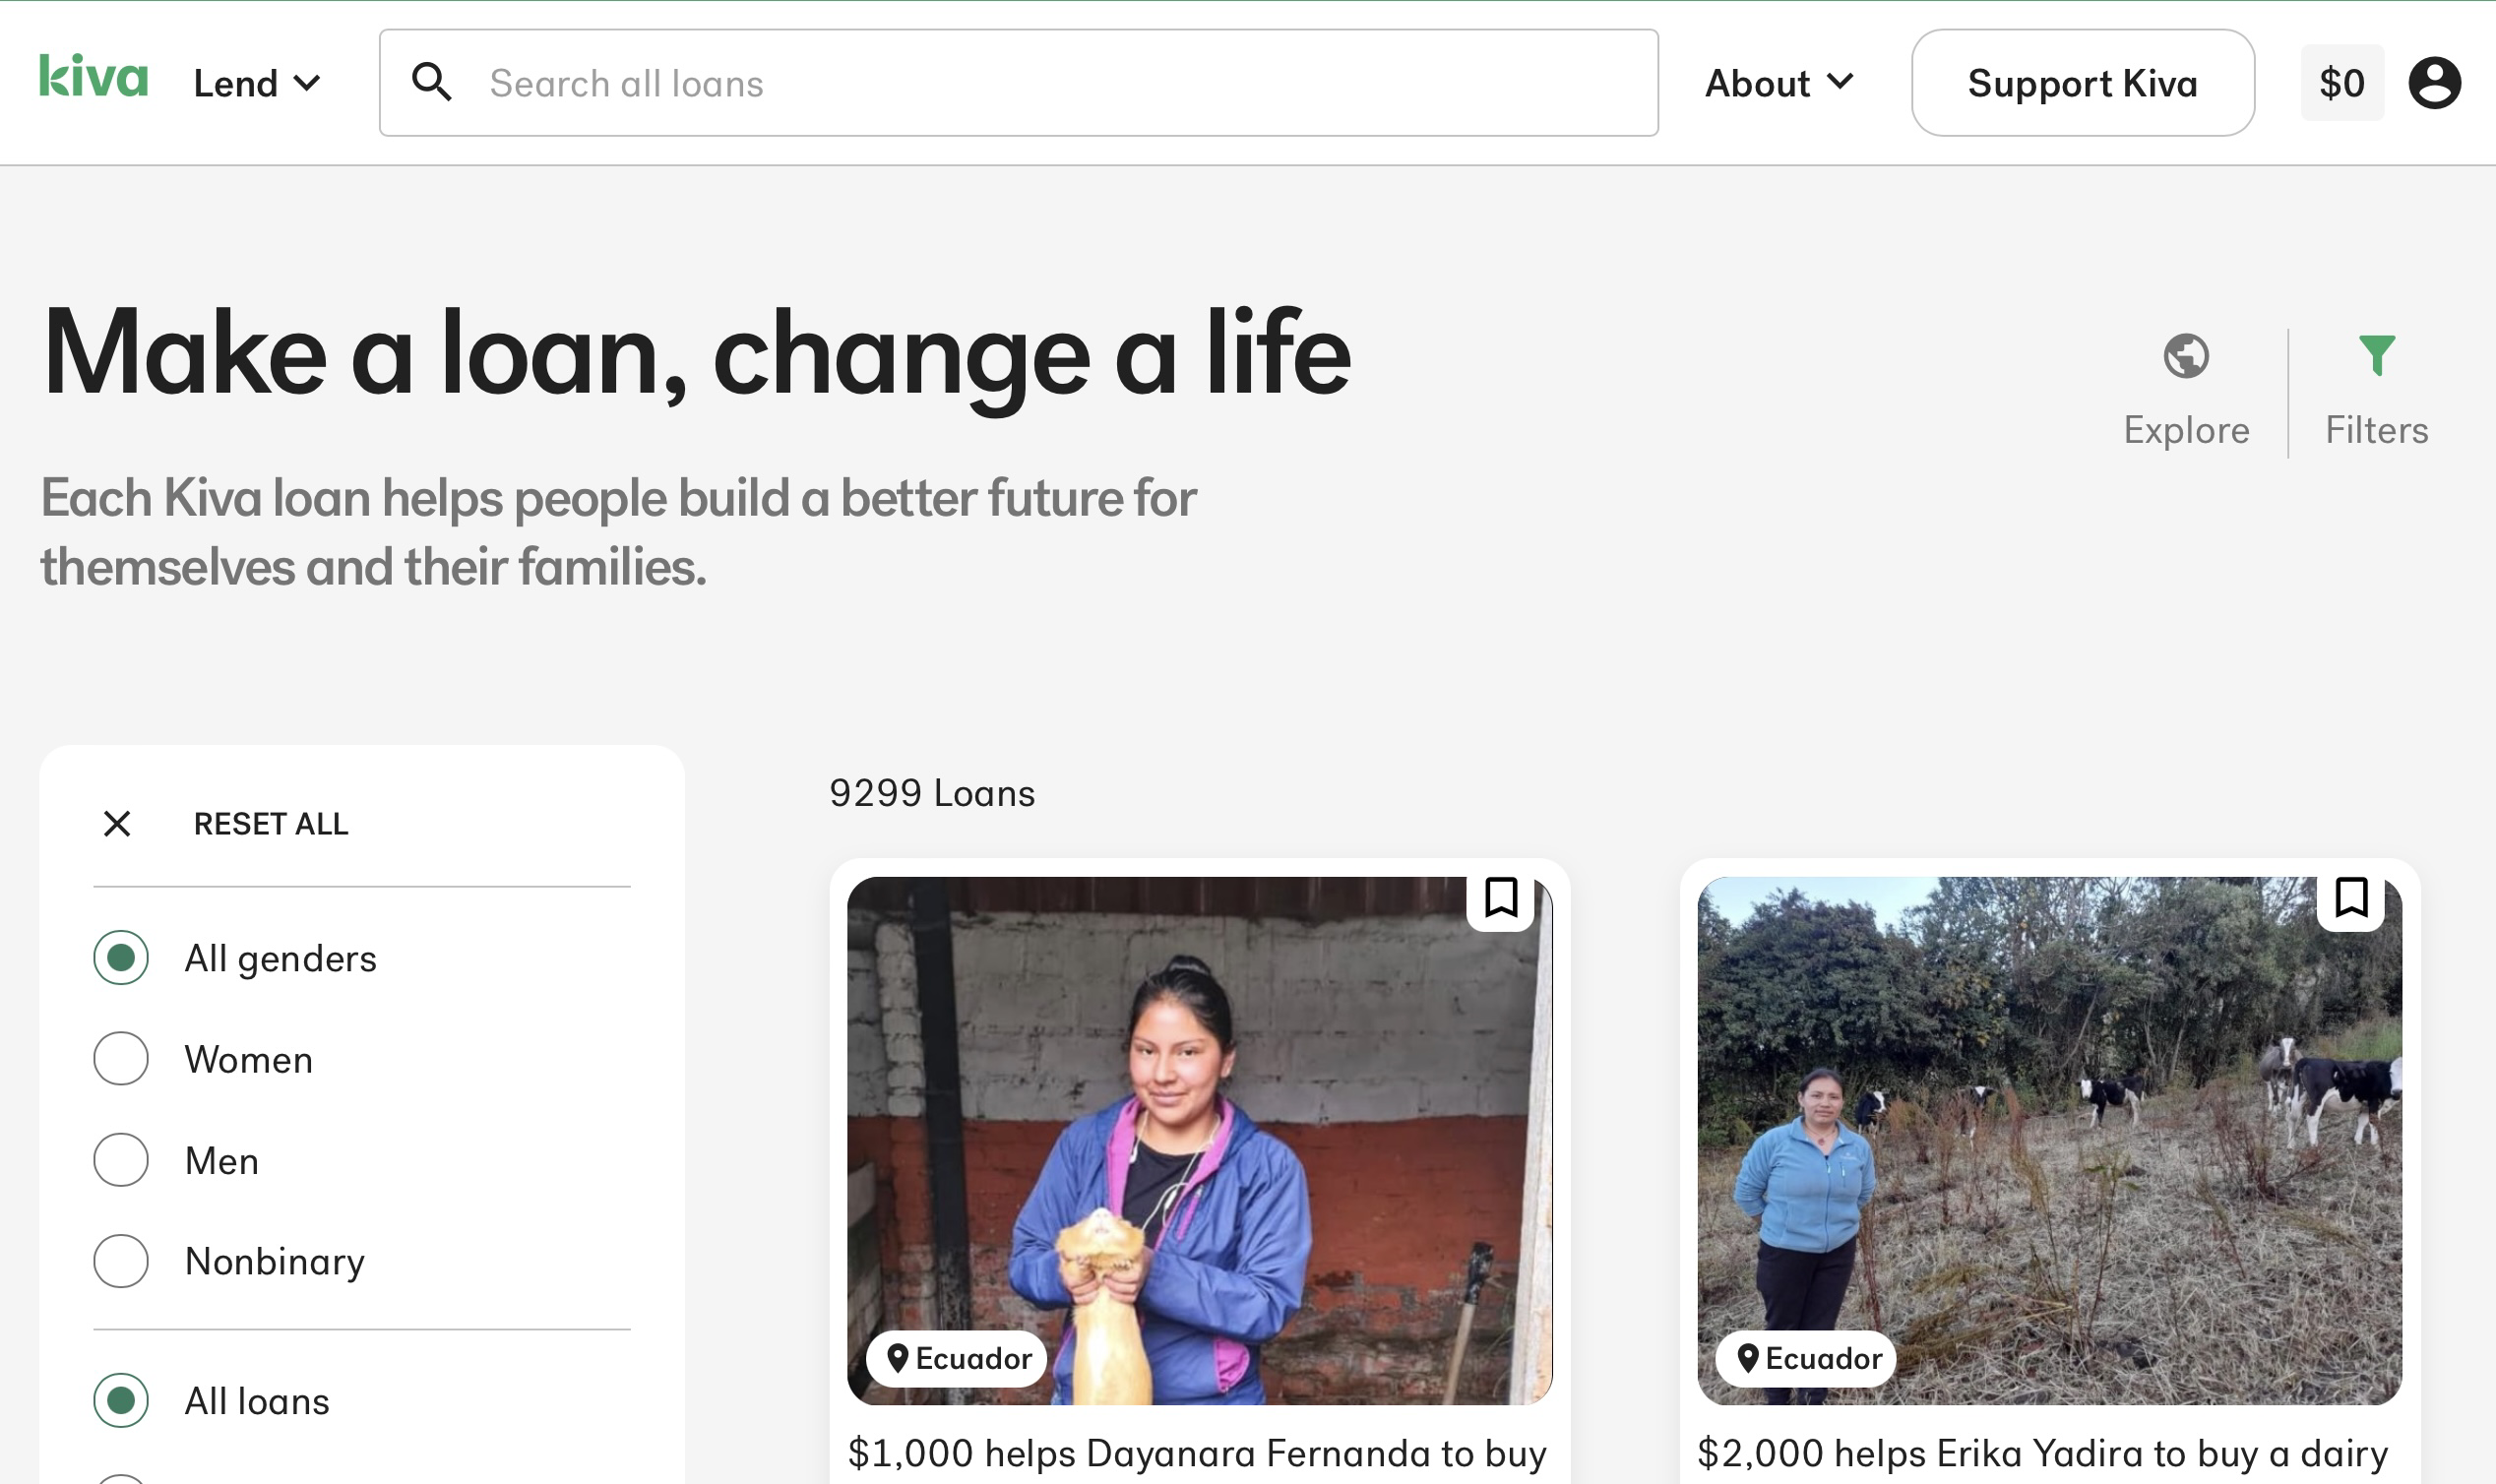
\includegraphics[width=0.8\textwidth]{images/kiva-browse-project.png}
	\caption{Kiva website interface for browsing projects}
	\label{fig:kiva-browser-project}
\end{figure}

It is important to know what Lenders can do when looking for his or her interested project.
Table \ref{tab:browser-criteria} shows the criteria that Lenders can use to filter the projects.
Later in the thesis, we will see that these criteria is not very align with the public data that the platform provide.
For example in the data, we could see some Tags that did not appear in the Tags list in the website.
We will consider these criteria as the gold standard for processing the data.

\begin{table}[H]
	\centering
	\resizebox{\textwidth}{!}{%
		\begin{tabular}{|c|c|c|c|}
			\hline
			   & Meaning                       & Type            & choices                                                                                                                 \\
			\hline
			1  & Gender of the borrower button & Choice          & Woman or Men or Nonbinary                                                                                               \\
			2  & Filter by type of Loan        & Choice          & Individual or Group                                                                                                     \\
			3  & Search by keyword             & Text            & Put any keyword to search in the stories of Projects                                                                    \\
			4  & Sort Order                    & Choice          & Amount: High to Low, Amount left, Amount: Low to High, Ending soon, Most recent, Trending now, Loan Length, Recommended \\
			5  & Location                      & Multiple choice & Choose from a list of countries                                                                                         \\
			6  & Sector                        & Multiple choice & Choose from a list of sectors                                                                                           \\
			7  & Attribute                     & Multiple choice & Choose from a list of attributes                                                                                        \\
			8  & Tags                          & Multiple choice & Choose from a list of tags                                                                                              \\
			9  & Loan Length                   & Choice          & All loans, 8 month or less, 16 months or less, 2 years or less, 2 years or more                                         \\
			10 & Loan Distribution             & Choice          & All loans, Parter, Direct                                                                                               \\
			11 & Partner Info                  & Text            & Search by Partner name                                                                                                  \\
			12 & Risk Rating                   & Range           & From 1 to 5                                                                                                             \\
			13 & Default Rate                  & Range           & From 0\% to 100\%                                                                                                       \\
			14 & Profitability                 & Range           & From -160\% to 90\%                                                                                                     \\
			\hline
		\end{tabular}%
	}
	\caption{Table with 4 columns \cite{kiva-browse}}
	\label{tab:browser-criteria}
\end{table}

Perhaps the most unique feature of Kiva is the Auto-Lending program.
In the program, Lenders can setup criterias for future projects that they want to fund.
When a new project is created, the platform will automatically fund the project if it fits the criterias.
Figure \ref{fig:auto-lend-setup} shows the interface for setting up the Auto-Lending program.

\begin{figure}[H]
	\centering
	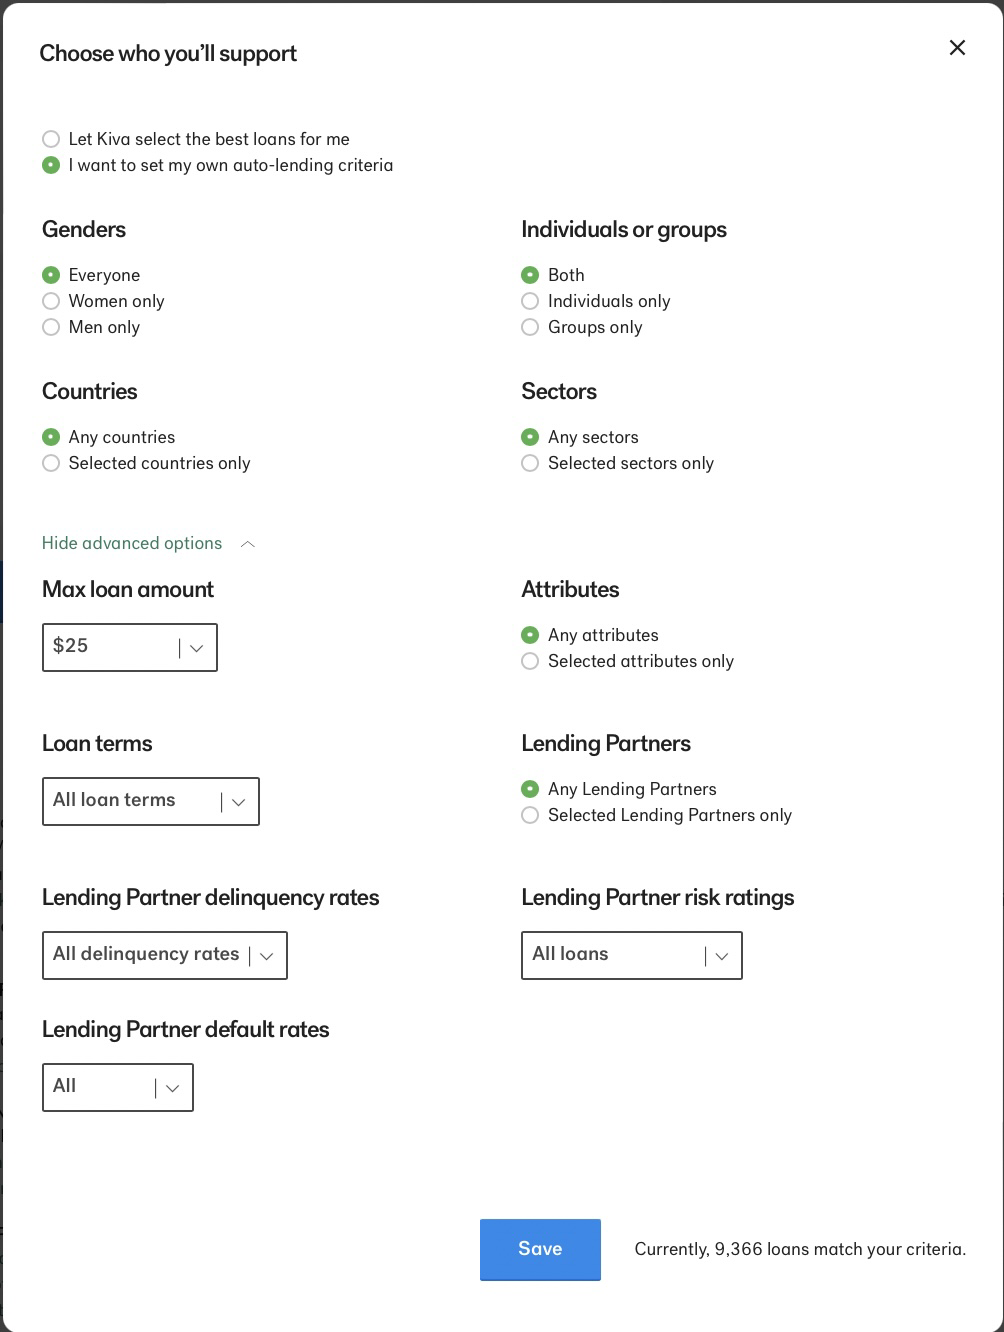
\includegraphics[width=0.8\textwidth]{images/auto-lend-setup.png}
	\caption{Auto-Lending setup interface \cite{kiva-autolend2}}
	\label{fig:auto-lend-setup}
\end{figure}

Users can "Let Kiva select the best loans for me" or "I want to set my own auto-lending criteria".
We do not have any information about how the platform select the best loans for users.
So we will focus on the second option.
We can see that the criterias are very similar to the criterias that users can use to search for projects.

\subsection{Kiva Data Access}

In order to access the data provided by Kiva, we utilize the GraphQL API.
Kiva has made their data available through this API, allowing developers to query and retrieve specific information from the platform.
This is perhap unique to Kiva, as most other crowdfunding platforms do not provide such access to their data.
It is also note that Kiva also provides a public dataset through their so called "Data Snapshot".
However, this function is appearantly not working at the time of writing.
There also another way to get the data from kiva website, which is through Web Crawling.
By analysis the website interface and the network traffic, we can get the data that the website use to display the information.
This approach is although popular, but it is not very reliable because the website can change its interface at any time.
In this thesis, we will focus on the GraphQL API.

GraphQL is a query language for APIs that provides a flexible and efficient way to request and manipulate data.
It allows us to specify the exact data we need and retrieve it in a single request, reducing the amount of network traffic and improving performance.
By leveraging the GraphQL API, we can easily access various data points such as borrower information, loan details, lender statistics, and more.
This enables us to perform in-depth analysis and gain valuable insights from the Kiva dataset.
The availability of Kiva's data through GraphQL provides us with a powerful tool to explore and analyze the platform's data in a convenient and efficient manner.

There are two noteworthy points about the GraphQL API.
The first is through the \textit{introspection} \cite{graphql-introspection} feature of GraphQL,
we could have the information of what queries that the platform supports,
as long as with the data schema.
The second is that we can ultilize the GraphQL API to get the data in a batched manner.
Usually the platform will limit the number of requests that a user can make to the API.
But if we use some Web Crawling techniques, we can manage to get all the data that avaliable in the API.

Kiva GraphQL API can be found publicly at \url{https://api.kivaws.org/graphql}.
One can connect to the URI with any compatible GraphQL client.
On top of that, kiva also use \textit{GraphQLi}, a web interface for easy try the GraphQL queries.
\ref{fig:grapqli} is the screenshot of the web interface.
We use the interface to introspection the data schema and to try out some queries before actually implementing them in the code.

\begin{figure}[H]
	\centering
	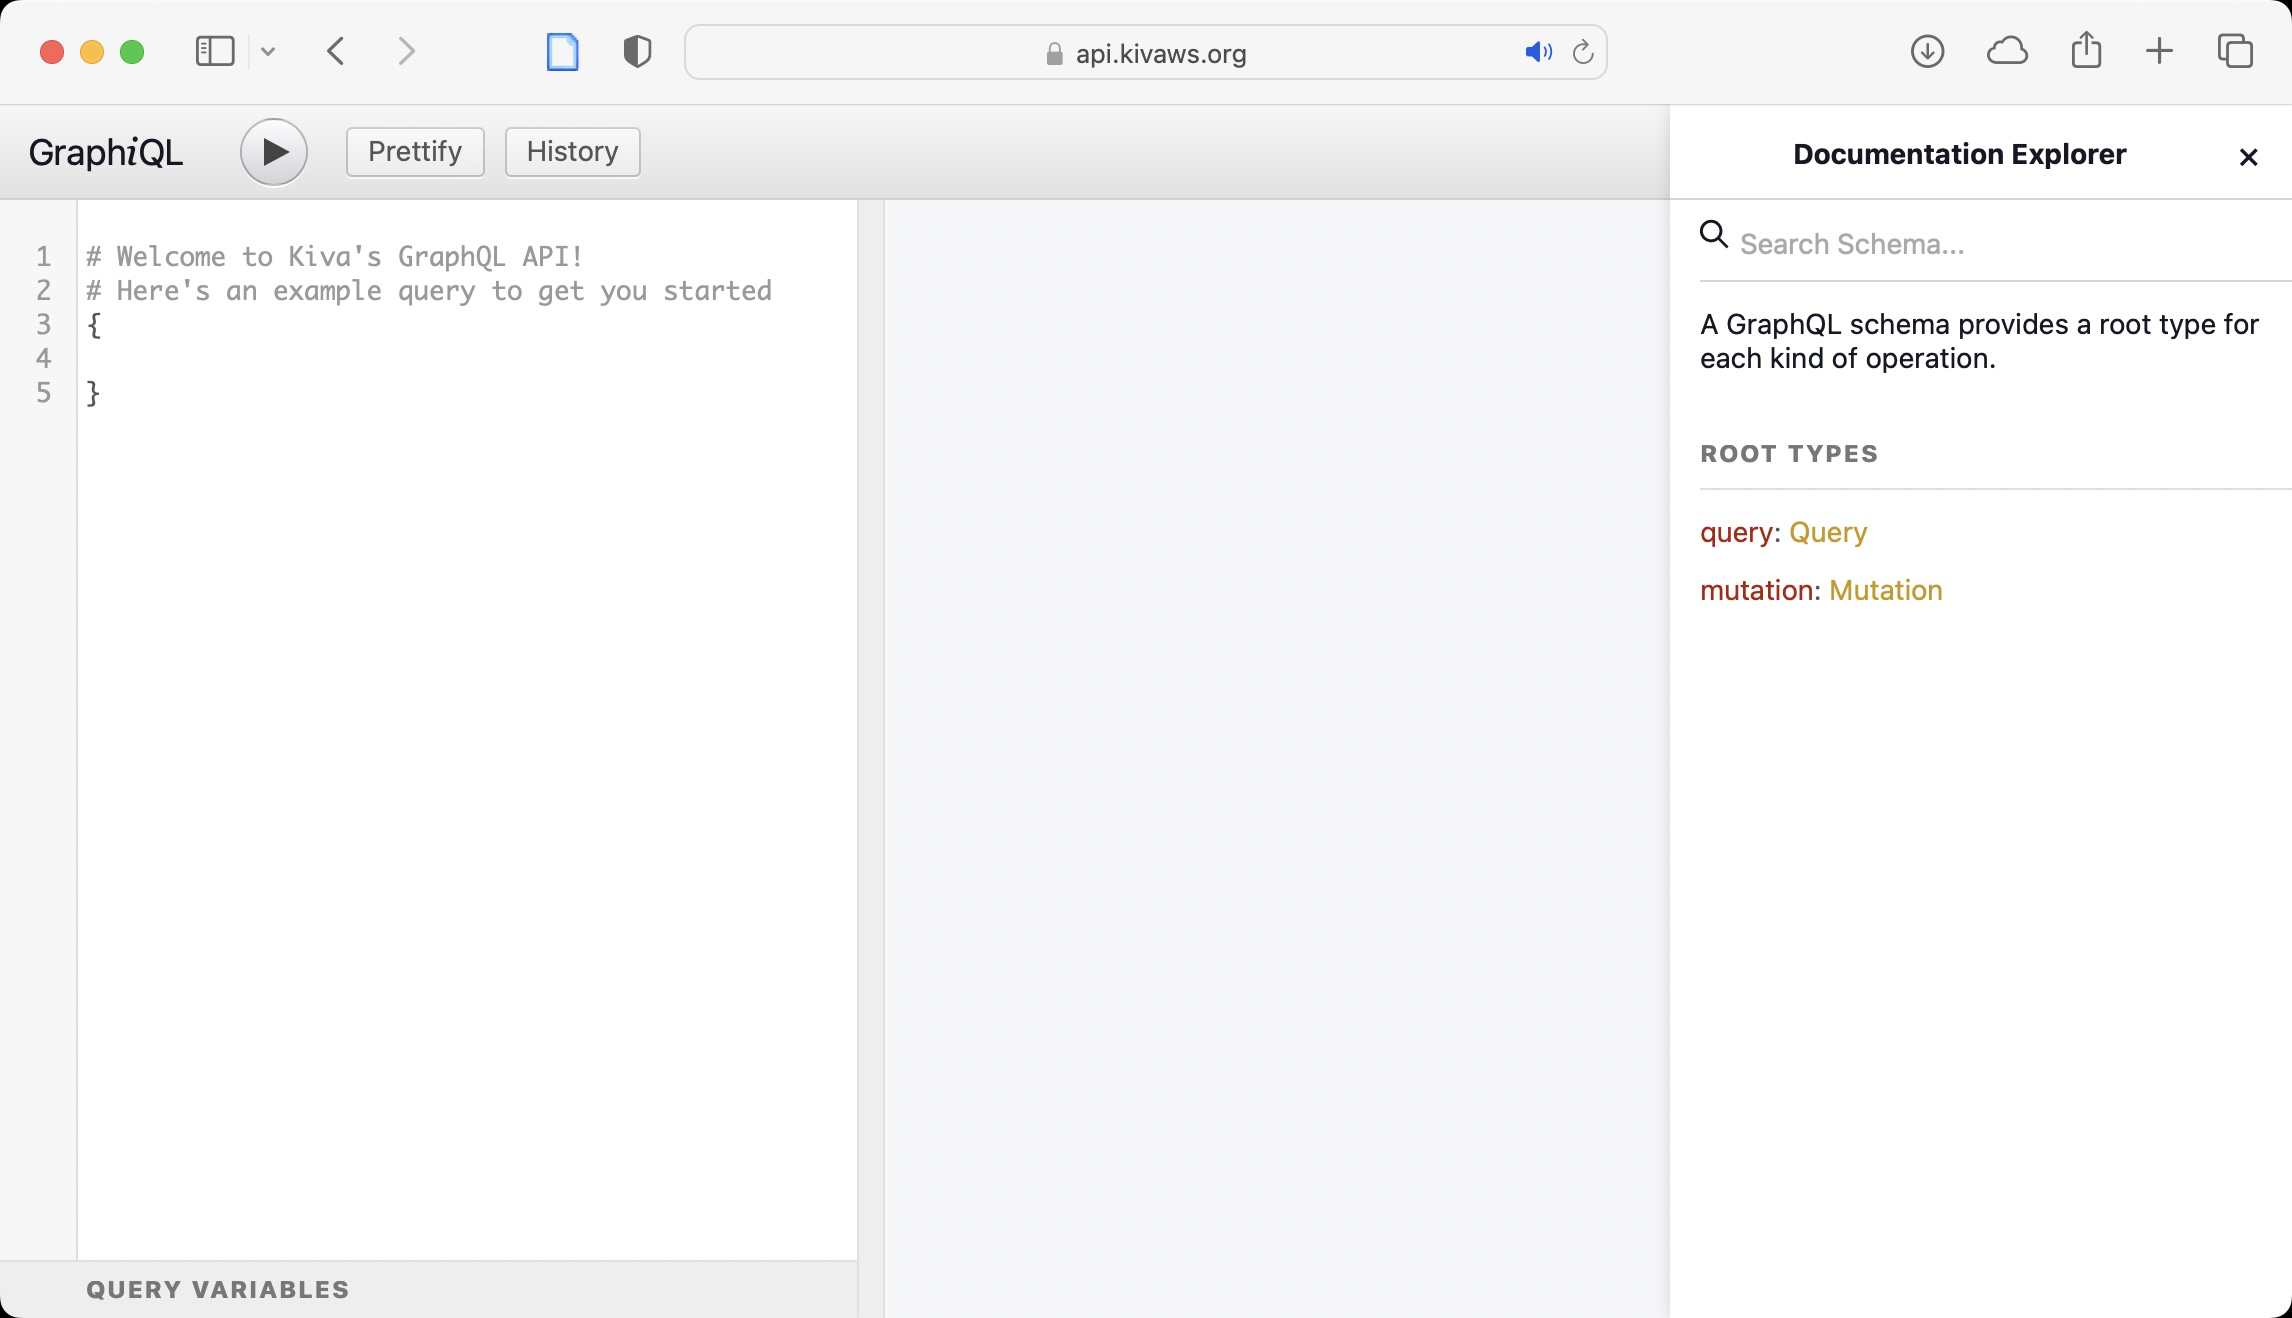
\includegraphics[width=0.8\textwidth]{images/grapqli.png}
	\caption{GraphQLi interface of Kiva GraphQL API}
	\label{fig:grapqli}
\end{figure}

For example, we could try the query for getting basic stats of kiva like following Figure \ref{fig:graphqli-example}.
One can use the Docs side bar (the right side bar) to discover what is the data that the API offer.
A basic knowledge about GraphQL would be helpful to discover the data schema more easily.

\begin{figure}[H]
	\centering
	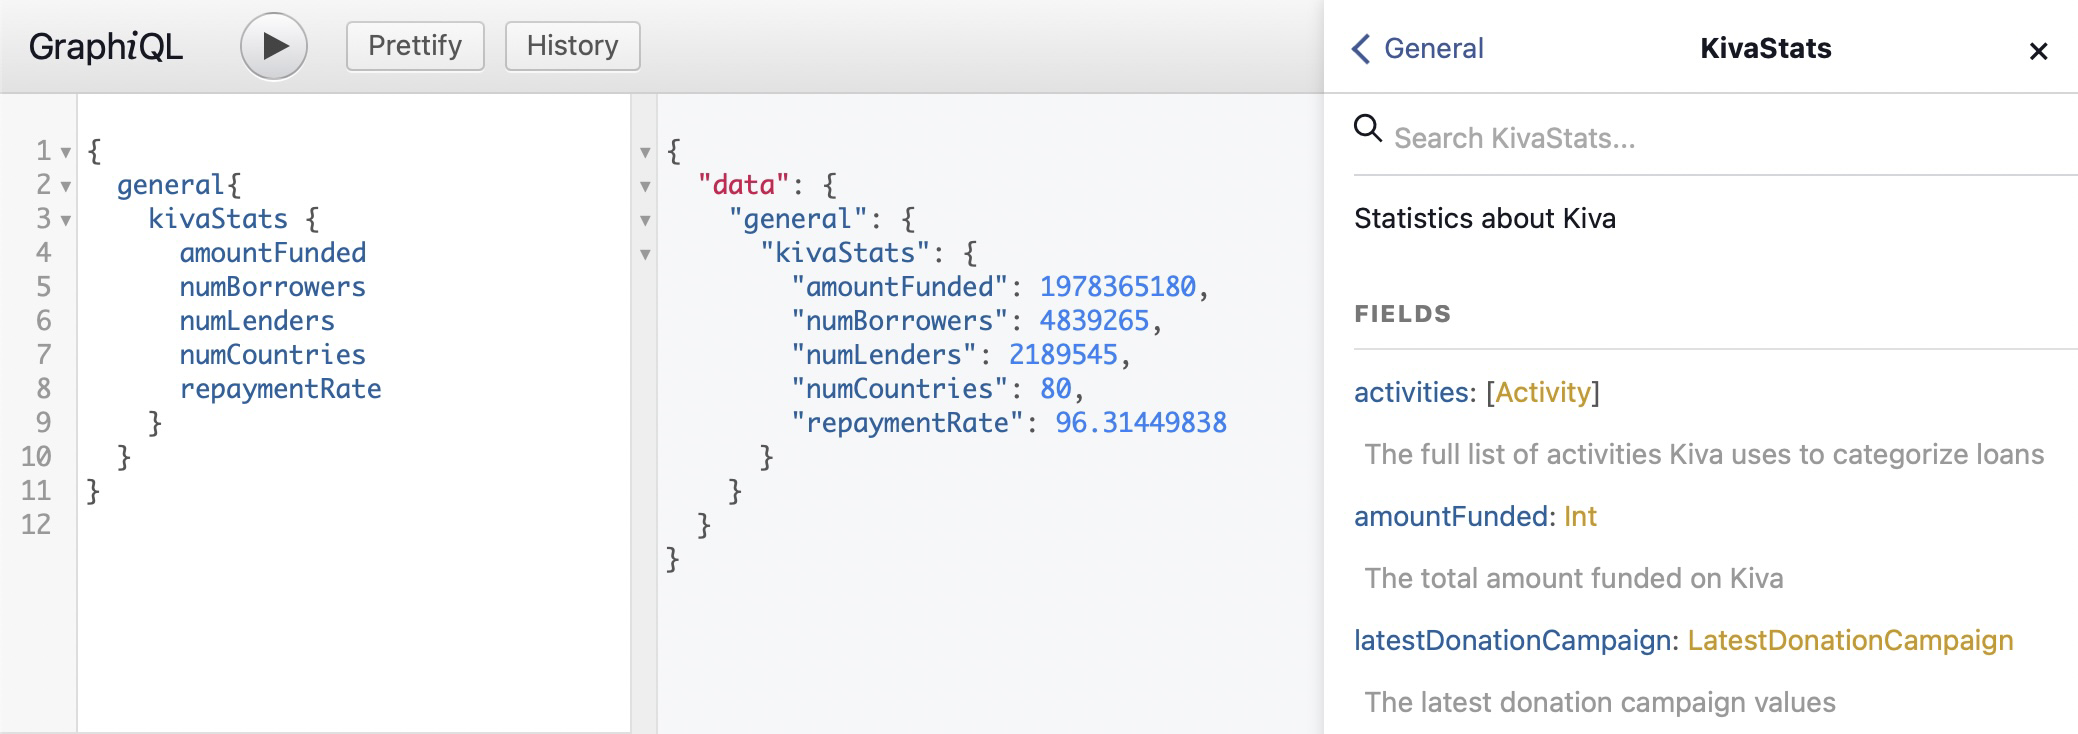
\includegraphics[width=0.8\textwidth]{images/graphqli-example.png}
	\caption{Example using GraphQLi interface of Kiva GraphQL API \cite{graphqli-example}}
	\label{fig:graphqli-example}
\end{figure}


Before begining to query the data, we have to understand the data schema to know what data that we can get.


\begin{figure}[H]
	\centering
	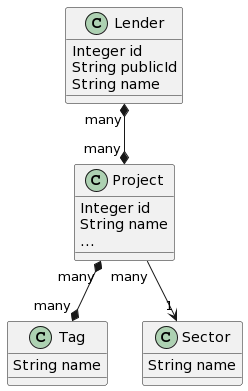
\includegraphics[width=0.25\textwidth]{images/graphuml/dataschema.png}
	\caption{Data schema}
	\label{fig:data-schema}
\end{figure}

The relationship beteen Lender and Project is many-to-many.
Each Project in Kiva can be funded by many Lenders.
And each Lender can fund many Projects.
The relationship between Project and Tag is also many-to-many.
The fields that we could get from each Project is described in Table \ref{tab:fields-meaning}.
We have to note that, in the APIs, kiva use the term "Loan" to indicate a single project.
We found it rather misunderstanding to use "Loan", so we try our best to use "Project" to avoid those misleading.
In this thesis, if a "Loan" appear (with the letter L in capital), one can understand the meaning is a "Project".


\begin{longtable}{|p{0.33\textwidth}|p{0.67\textwidth}|}
	\toprule\noalign{}
	\caption{Fields of Projects}
	\label{tab:fields-meaning}                                                                               \\

	\hline
	\multicolumn{1}{|c|}{\textbf{Field}} & \multicolumn{1}{c|}{\textbf{Meaning}}                             \\
	\hline
	\endfirsthead

	\multicolumn{2}{c}%
	{{\bfseries \tablename\ \thetable{} -- continued from previous page}}                                    \\
	\hline
	\multicolumn{1}{|c|}{\textbf{Field}} & \multicolumn{1}{c|}{\textbf{Meaning}}                             \\
	\hline
	\endhead

	\hline
	\multicolumn{2}{|r|}{{Continued on next page}}                                                           \\ \hline
	\endfoot

	\hline \hline
	\endlastfoot

	activity                             & The activity is a structured categorization of the loan
	use                                                                                                      \\
	anonymizationLevel                   & The level of borrower privacy                                     \\
	borrowerCount                        & The number of borrowers participating in the loan                 \\
	borrowers                            & The one or more borrowers that are receiving this loan. If
	there is more than one, the primary borrower is first                                                    \\
	dafEligible                          & Whether or not the loan is eligible for donor-advised
	funds.                                                                                                   \\
	delinquent                           & Whether or not the loan is delinquent. This defaults to
	false if the user is not privileged to this loan                                                         \\
	description                          & The description of the loan profile in English.                   \\
	descriptionInOriginalLanguage        & The description of the loan profile in
	the original language of its posting                                                                     \\
	disbursalDate                        & The date on which the loan was/will actually be
	disbursed to the borrower                                                                                \\
	distributionModel                    & How the loan is distributed to the borrower,
	e.g.~`field\_partner' or `direct'                                                                        \\
	endorser                             & The user who endorsed the loan. Only shown on fundRaising
	loans, null for all other statuses.                                                                      \\
	fundraisingDate                      & When the loan started fundraising on Kiva. Same as
	posted\_date in v1.                                                                                      \\
	gender                               & The gender of the primary borrower OR majority gender if
	group                                                                                                    \\
	geocode                              & The physical location of the borrower and/or business             \\
	hasCurrencyExchangeLossLenders       & Whether or not the loan has currency
	loss to lenders. Only usable after the loan has moved into the ``ended''
	state.                                                                                                   \\
	id                                   & Unique identifier for a Kiva loan                                 \\
	image                                & The picture for this loan profile.                                \\
	isMatchable                          & Is this Kiva loan matchable? e.g.~is there a source of
	funds to provide matching if a share is purchased?                                                       \\
	inPfp                                & If true, this loan is in a Private Fundraising Period             \\
	loanAmount                           & The amount of this loan, as shown to lenders                      \\
	loanFundraisingInfo                  & Information about this loan during its fundraising
	period                                                                                                   \\
	lenderRepaymentTerm                  & The number of months it will take the borrower to
	repay the loan                                                                                           \\
	matcherAccountId                     & The id of the loan matcher                                        \\
	matcherName                          & The name of the loan matcher                                      \\
	matchRatio                           & The loan match ratio                                              \\
	matchingText                         & Text that is displayed if loan matching is turned on for
	this loan.                                                                                               \\
	name                                 & The name of the borrower or group receiving the loan              \\
	originalLanguage                     & The original language on the loan                                 \\
	minNoteSize                          & The minimum amount to lend for this loan                          \\
	paidAmount                           & The amount of settled repayments for a loan that has
	started paying back                                                                                      \\
	pfpMinLenders                        & The minimum number of lenders that this loan needs to
	exit its private fundraising period (PFP).                                                               \\
	plannedExpirationDate                & When the loan will expire if it is not fully
	funded                                                                                                   \\
	previousLoanId                       & ID of the loan linked as previous to this one.                    \\
	raisedDate                           & When the loan became raised, e.g.~fully funded. Same as
	funded\_date in v1                                                                                       \\
	researchScore                        & The research score of the loan theme instance of the
	loan                                                                                                     \\
	repaymentInterval                    & The repayment interval of the loan: ``monthly'',
	``irregularly'',``at\_end''                                                                              \\
	sector                               & The sector is a more general classification of the loan than
	activity                                                                                                 \\
	status                               & The status of a loan                                              \\
	tags                                 & A list of tags on this loan                                       \\
	terms                                & The financial terms of this loan                                  \\
	use                                  & Text describing what the loan is to be used for; a logical subset
	of description e.g.~``To buy a cow''                                                                     \\
	userProperties                       & Properties that apply to the logged in user in relation
	to a loan.                                                                                               \\
	video                                & Video for this loan                                               \\
	whySpecial                           & Why this loan is considered special.                              \\
	comments                             & List of A user comment made on a Kiva loan.                       \\
	lenders                              & List of Representation of a Kiva lender                           \\
	lendingActions                       & List of Representation of a lending action                        \\
	teams                                & List of Representation of a Kiva lending team                     \\
\end{longtable}

The example data that we get from the API is shown in Table \ref{tab:example-data}.

\begin{longtable}{|p{0.36\textwidth}|p{0.64\textwidth}|}
	\toprule\noalign{}
	\caption{An Example Project}
	\label{tab:example-data}                                                                                              \\

	\hline
	\multicolumn{1}{|c|}{\textbf{Field}}            & \multicolumn{1}{c|}{\textbf{Meaning}}                               \\
	\hline
	\endfirsthead

	\multicolumn{2}{c}%
	{{\bfseries \tablename\ \thetable{} -- continued from previous page}}                                                 \\
	\hline
	\multicolumn{1}{|c|}{\textbf{Field}}            & \multicolumn{1}{c|}{\textbf{Meaning}}                               \\
	\hline
	\endhead

	\hline
	\multicolumn{2}{|r|}{{Continued on next page}}                                                                        \\
	\hline
	\endfoot

	\hline \hline
	\endlastfoot

	anonymizationLevel                              & none                                                                \\
	borrowerCount                                   & 1                                                                   \\
	borrowers                                       & {[}\{`id': 2843387, `borrowedAmount': `440.80', `firstName':
	`Jessenia Elizabeth', `gender': `female', `isPrimary': True, `pictured':
	True\}{]}                                                                                                             \\
	dafEligible                                     & False                                                               \\
	delinquent                                      & False                                                               \\
	disbursalDate                                   & 2013-09-25T07:00:00Z                                                \\
	distributionModel                               & fieldPartner                                                        \\
	endorser                                        &                                                                     \\
	fundraisingDate                                 & 2013-10-23T22:40:01Z                                                \\
	gender                                          & female                                                              \\
	hasCurrencyExchangeLossLenders                  & False                                                               \\
	id                                              & 623042                                                              \\
	isMatchable                                     & False                                                               \\
	inPfp                                           & False                                                               \\
	loanAmount                                      & 450.00                                                              \\
	lenderRepaymentTerm                             & 8                                                                   \\
	matcherAccountId                                &                                                                     \\
	matcherName                                     &                                                                     \\
	matchRatio                                      &                                                                     \\
	matchingText                                    &                                                                     \\
	name                                            & Jessenia Elizabeth                                                  \\
	minNoteSize                                     & 25.00                                                               \\
	paidAmount                                      & 0.00                                                                \\
	pfpMinLenders                                   &                                                                     \\
	plannedExpirationDate                           & 2013-11-22T22:40:01Z                                                \\
	previousLoanId                                  &                                                                     \\
	raisedDate                                      & 2013-10-24T13:38:51Z                                                \\
	researchScore                                   & 9                                                                   \\
	repaymentInterval                               & monthly                                                             \\
	status                                          & funded                                                              \\
	tags                                            & {[}{]}                                                              \\
	use                                             & purchase school supplies and other stationery items for her
	store.                                                                                                                \\
	video                                           &                                                                     \\
	whySpecial                                      &                                                                     \\
	activity.id                                     & 103                                                                 \\
	activity.name                                   & Paper Sales                                                         \\
	geocode.city                                    & Pichincha                                                           \\
	geocode.state                                   & Pichincha                                                           \\
	geocode.country.name                            & Ecuador                                                             \\
	geocode.country.isoCode                         & EC                                                                  \\
	geocode.country.region                          & South America                                                       \\
	geocode.country.ppp                             & \$10,600                                                            \\
	geocode.country.\densetext{numLoansFundraising} & 553                                                                 \\
	geocode.country.fundsLentInCountry              & 87573245                                                            \\
	geocode.postalCode                              &                                                                     \\
	geocode.latitude                                & -0.1464847                                                          \\
	geocode.longitude                               & -78.4751945                                                         \\
	image.id                                        & 1456025                                                             \\
	image.url                                       &
	https://www-kiva-org-0.freetls.fastly.net/img/s100/5cf86ba6c72db94f0721b934a57ca889.jpg                               \\
	loanFundraisingInfo.fundedAmount                & 450.00                                                              \\
	loanFundraisingInfo.isExpiringSoon              & False                                                               \\
	loanFundraisingInfo.reservedAmount              & 0.00                                                                \\
	originalLanguage.id                             & 2                                                                   \\
	originalLanguage.isActive                       & True                                                                \\
	originalLanguage.isoCode                        & ES                                                                  \\
	originalLanguage.name                           & Spanish                                                             \\
	sector.id                                       & 7                                                                   \\
	sector.name                                     & Retail                                                              \\
	terms.currency                                  & USD                                                                 \\
	terms.currencyFullName                          & United States Dollars                                               \\
	terms.disbursalAmount                           & 440.80                                                              \\
	terms.disbursalDate                             & 2013-09-25T07:00:00Z                                                \\
	terms.expectedPayments                          & {[}{]}                                                              \\
	terms.loanAmount                                & 450.00                                                              \\
	terms.lenderRepaymentTerm                       & 8                                                                   \\
	terms.lossLiabilityCurrencyExchange             & none                                                                \\
	terms.lossLiabilityNonpayment                   & lender                                                              \\
	terms.flexibleFundraisingEnabled                & False                                                               \\
	userProperties.favorited                        &                                                                     \\
	userProperties.lentTo                           &                                                                     \\
	userProperties.subscribed                       &                                                                     \\
	userProperties.promoEligible                    & False                                                               \\
	userProperties.amountInBasket                   &                                                                     \\
	lendingActions.totalCount                       & 14                                                                  \\
	lendingActions.values                           & {[}\{`lender': \{`id': 32817, `name': `Nate',
	`publicId': `nateinaction'\}, `shareAmount': `25.00', `teams': {[}`(A+)
	Atheists'{]}, `latestSharePurchaseDate': `2013-10-24T11:50:07Z'\},
	\{`lender': \{`id': 55596, `name': `Dirk L.', `publicId': `DirkLebe'\},
	`shareAmount': `25.00', `teams': {[}{]}, `latestSharePurchaseDate':
	`2013-10-24T02:40:53Z'\}{]}                                                                                           \\
	description                                     & Every fifteen days, the members of the Community Bank of
	Pichincha meet in their home region of Pichincha. This area is well
	known as a vibrant place, where the majority of the people are farmers
	or ranchers. It's a highly vegetated area, cut by a great river that
	nurtures the crops.                                                                                                   \\
	                                                & This is where Jessenia, 27 years old, lives with her common-law
	husband and their three children, aged 9, 4, and 2 years. The eldest is
	a student, and her husband is a shopkeeper.Jessenia is a woman with
	spirit who likes to work to get ahead. For the last six years, she has
	run a shop out of her home that functions as a stationery shop and a
	bookstore. Day by day, the store has improved. Currently, apart from
	books and supplies, she also sells trinkets and other school/office
	supplies. With these products, her earnings have greatly increased, and
	thanks to the loans she has received, she has been able to expand her
	business.                                                                                                             \\
	                                                & This loan will be used to buy school supplies and other stationery
	products. She has been in the Community Bank for eight years and she
	likes it because the loans have helped her improve her business. She
	dreams of expanding it further still.                                                                                 \\
	descriptionInOriginalLanguage                   & En el cantón Pichincha cada quince días
	se reúne el Banco Comunal Pichincha, este lugar se lo conoce por ser muy
	dinámico donde la mayoría de sus habitantes se dedican a la agricultura
	y a la cría de animales, por ser una zona con gran vegetación surcada
	por un gran rio lo cual lo hace propicia para los cultivos.                                                           \\
	                                                & En este lugar vive la señora Jessenia, tiene 27 años de edad y
	mantiene una relación de unión libre de la cual tiene tres hijos de 9, 4
	y 2 años de edad, el mayor estudia en escuela. El marido es
	comerciante.                                                                                                          \\
	                                                & Doña Jessenia es una mujer muy luchadora que le gusta trabajar para
	salir adelante, ella hace mas de 6 años adecuo un local en su casa y en
	el mismo instaló una papelería y librería, la misma que con el paso de
	los días ha ido mejorando, actualmente además de libros y útiles también
	vende bisutería y artículos de bazar con esto sus ganancias han mejorado
	mucho y esto gracias a los créditos que ha recibido ya que con ellos
	cada vez aumenta más su negocio.                                                                                      \\
	                                                & Este crédito es para comprar útiles escolares y artículos de bazar.
	Esta desde hace 8 años en el Banco Comunal y le gusta porque los
	créditos le han ayudado a mejora su negocio. Sus sueños son aumentar más
	su negocio.                                                                                                           \\
\end{longtable}

Recall that when browse and search for Project in the kiva website,
users can filter Projects by Sectors, Activities, Attributes, Tags.
The API document provide a good definition for some of those terms.

\textbf{Sector}

From the API documentation, we have the definition of Sector as, quoted:
"A sector is a broad category for a loan, e.g. Agriculture, Arts, Clothing. Sectors are subdivided further by activities."
We take a step further to get all the possible Sectors that the platform support,
this can be done using the following GraphQL query:

\begin{lstlisting}
    {
        lend {
            sector {
                id
                name
            }
        }
    }
\end{lstlisting}

The result is shown in Table \ref{tab:sector-definition}.

\begin{longtable}[]{@{}rl@{}}
	\caption{Definition of Sectors}
	\label{tab:sector-definition} \\
	\toprule\noalign{}
	id & name                     \\
	\midrule\noalign{}
	\endhead
	\bottomrule\noalign{}
	\endlastfoot
	1  & Agriculture              \\
	3  & Transportation           \\
	4  & Services                 \\
	5  & Clothing                 \\
	6  & Health                   \\
	7  & Retail                   \\
	8  & Manufacturing            \\
	9  & Arts                     \\
	10 & Housing                  \\
	12 & Food                     \\
	13 & Wholesale                \\
	14 & Construction             \\
	15 & Education                \\
	16 & Personal Use             \\
	17 & Entertainment            \\
\end{longtable}

\textbf{Activity}

"A property of loan which is more descriptive than Sector.
Every activity is within a sector. e.g. the 'Animal Sales' activity is within the 'Agriculture' sector.
Note, some Activities have the same name as their parent Sector."
Quoted from the API documentation.
All the possible Activities can be found using the following GraphQL query:

\begin{lstlisting}
    {
        lend {
            activity {
                id
                name
                }	
        }
    }
\end{lstlisting}

The result is show in Table \ref{tab:activity-definition}.

\begin{longtable}[]{|r|l|r|l|r|l|}

	\toprule\noalign{}
	\caption{Definition of Activities}
	\label{tab:activity-definition}                                                                                                                                                                                          \\

	\hline
	\multicolumn{1}{|c|}{\textbf{id}} & \multicolumn{1}{c|}{\textbf{Name}} & \multicolumn{1}{|c|}{\textbf{id}} & \multicolumn{1}{c|}{\textbf{Name}} & \multicolumn{1}{|c|}{\textbf{id}} & \multicolumn{1}{c|}{\textbf{Name}} \\
	\hline
	\endfirsthead

	\multicolumn{6}{c}%
	{{\bfseries \tablename\ \thetable{} -- continued from previous page}}                                                                                                                                                    \\
	\hline
	\multicolumn{1}{|c|}{\textbf{id}} & \multicolumn{1}{c|}{\textbf{Name}} & \multicolumn{1}{|c|}{\textbf{id}} & \multicolumn{1}{c|}{\textbf{Name}} & \multicolumn{1}{|c|}{\textbf{id}} & \multicolumn{1}{c|}{\textbf{Name}} \\
	\hline
	\endhead

	\hline
	\multicolumn{6}{|r|}{{Continued on next page}}                                                                                                                                                                           \\
	\hline
	\endfoot

	\hline \hline
	\endlastfoot


	9                                 & Clothing Sales                     & 84                                & Used Clothing                      & 147                               & Well digging                       \\
	11                                & Land Rental                        & 85                                & Laundry                            & 149                               & Embroidery                         \\
	12                                & Traveling Sales                    & 86                                & Textiles                           & 151                               & Music Discs \& Tapes               \\
	13                                & Veterinary Sales                   & 87                                & Food Market                        & 156                               & Rickshaw                           \\
	14                                & Bookstore                          & 88                                & Retail                             & 157                               & Call Center                        \\
	15                                & Grocery Store                      & 89                                & Fishing                            & 158                               & Primary/secondary school
	costs                                                                                                                                                                                                                    \\
	17                                & Musical Performance                & 91                                & Milk Sales                         & 159                               & Bookbinding                        \\
	18                                & Water Distribution                 & 92                                & Auto Repair                        & 161                               & Movie Tapes \&
	DVDs                                                                                                                                                                                                                     \\
	19                                & Cosmetics Sales                    & 94                                & Pub                                & 162                               & Liquor Store / Off-License         \\
	21                                & Bicycle Repair                     & 95                                & Machine Shop                       & 163                               & Waste Management                   \\
	23                                & Shoe Sales                         & 96                                & Phone Accessories                  & 164                               & Film                               \\
	24                                & Construction Supplies              & 97                                & Cement                             & 165                               & Knitting                           \\
	25                                & Cafe                               & 98                                & Decorations Sales                  & 167                               & Upholstery                         \\
	26                                & Plastics Sales                     & 99                                & Pigs                               & 169                               & Fruits \& Vegetables               \\
	27                                & Bakery                             & 100                               & Phone Repair                       & 170                               & Jewelry                            \\
	28                                & Barber Shop                        & 101                               & Cobbler                            & 171                               & Cloth \& Dressmaking
	Supplies                                                                                                                                                                                                                 \\
	29                                & Home Products Sales                & 102                               & Poultry                            & 172                               & Internet Cafe                      \\
	31                                & Farming                            & 103                               & Paper Sales                        & 174                               & Entertainment                      \\
	32                                & Tailoring                          & 104                               & Electronics Repair                 & 175                               & Games                              \\
	33                                & Furniture Making                   & 105                               & Air Conditioning                   & 176                               & Education
	provider                                                                                                                                                                                                                 \\
	34                                & Butcher Shop                       & 107                               & Transportation                     & 177                               & Flowers                            \\
	35                                & Cheese Making                      & 108                               & Blacksmith                         & 180                               & Wholesale                          \\
	37                                & Motorcycle Transport               & 109                               & Perfumes                           & 181                               & Food                               \\
	39                                & Construction                       & 110                               & Animal Sales                       & 183                               & Clothing                           \\
	40                                & Phone Use Sales                    & 111                               & Computers                          & 184                               & Machinery Rental                   \\
	41                                & Sporting Good Sales                & 112                               & Cereals                            & 185                               & Food Stall                         \\
	43                                & Carpentry                          & 114                               & Secretarial Services               & 186                               & Balut-Making                       \\
	45                                & Catering                           & 115                               & Dental                             & 192                               & Personal Medical Expenses          \\
	46                                & Restaurant                         & 116                               & Electrician                        & 193                               & Property                           \\
	47                                & Sewing                             & 117                               & Mobile Phones                      & 194                               & Consumer Goods                     \\
	49                                & Beauty Salon                       & 119                               & Quarrying                          & 195                               & Home Appliances                    \\
	51                                & Electronics Sales                  & 120                               & Agriculture                        & 196                               & Vehicle                            \\
	52                                & Metal Shop                         & 121                               & Services                           & 197                               & Wedding Expenses                   \\
	54                                & Vehicle Repairs                    & 123                               & Health                             & 199                               & Used Shoes                         \\
	56                                & Cattle                             & 124                               & Manufacturing                      & 200                               & Higher education costs             \\
	57                                & General Store                      & 125                               & Arts                               & 201                               & Renewable Energy Products          \\
	59                                & Taxi                               & 127                               & Party Supplies                     & 202                               & Recycled Materials                 \\
	60                                & Charcoal Sales                     & 128                               & Timber Sales                       & 203                               & Home Energy                        \\
	61                                & Dairy                              & 129                               & Child Care                         & 204                               & Cleaning Services                  \\
	62                                & Photography                        & 130                               & Fuel/Firewood                      & 206                               & Communications                     \\
	63                                & Fish Selling                       & 131                               & Electrical Goods                   & 207                               & Adult Care                         \\
	65                                & Pharmacy                           & 132                               & Religious Articles                 & 208                               & Energy                             \\
	66                                & Printing                           & 133                               & Tourism                            & 209                               & Florist                            \\
	67                                & Food Production/Sales              & 134                               & Personal Housing Expenses          & 210                               &
	Landscaping / Gardening                                                                                                                                                                                                  \\
	68                                & Farm Supplies                      & 135                               & Motorcycle Repair                  & 216                               & Technology                         \\
	70                                & Medical Clinic                     & 137                               & Utilities                          & 217                               & Beekeeping                         \\
	72                                & Crafts                             & 138                               & Recycling                          & 218                               & Aquaculture                        \\
	73                                & Livestock                          & 140                               & Souvenir Sales                     & 219                               & Computer                           \\
	75                                & Patchwork                          & 141                               & Spare Parts                        & 220                               & Beverages                          \\
	76                                & Bicycle Sales                      & 142                               & Personal Products Sales            & 221                               & Personal Care
	Products                                                                                                                                                                                                                 \\
	78                                & Musical Instruments                & 143                               & Natural Medicines                  & 222                               & Funerals                           \\
	79                                & Bricks                             & 144                               & Goods Distribution                 & 223                               & Celebrations                       \\
	80                                & Office Supplies                    & 145                               & Weaving                            & 224                               & Personal Expenses                  \\
	81                                & Hardware                           & 146                               & Hotel                              & 225                               & Mobile Transactions                \\
	                                  &                                    &                                   &                                    & 226                               & Event Planning                     \\
\end{longtable}

\textbf{Tag}

The API give the definition of Tag as,
quoted: "Loan properties which are attributed by lenders"
With the following GraphQL query, we can get all the possible Tags that the platform support.

\begin{lstlisting}
    {
        lend {
            tag {
                id, # Unique identifier for this tag
                name, # The name of the tag
                vocabularyId # Vocabulary id for the tag type
            }
        }
    }
\end{lstlisting}

The result is shown in Table \ref{tab:tag-definition}.

\begin{longtable}{|r|l|l|r|l|l|}
	\toprule\noalign{}
	\caption{Definition of tags}
	\label{tab:tag-definition}                                                                                                                                                                                                                                         \\

	\hline
	\multicolumn{1}{|c|}{\textbf{id}} & \multicolumn{1}{c|}{\textbf{name}} & \multicolumn{1}{|c|}{\densetext{\textbf{vocabularyId}}} & \multicolumn{1}{c|}{\textbf{id}} & \multicolumn{1}{|c|}{\textbf{name}} & \multicolumn{1}{c|}{\densetext{\textbf{vocabularyId}}} \\
	\hline
	\endfirsthead

	\multicolumn{6}{c}%
	{{\bfseries \tablename\ \thetable{} -- continued from previous page}}                                                                                                                                                                                              \\
	\hline
	\multicolumn{1}{|c|}{\textbf{id}} & \multicolumn{1}{c|}{\textbf{name}} & \multicolumn{1}{|c|}{\densetext{\textbf{vocabularyId}}} & \multicolumn{1}{c|}{\textbf{id}} & \multicolumn{1}{|c|}{\textbf{name}} & \multicolumn{1}{c|}{\densetext{\textbf{vocabularyId}}} \\
	\hline
	\endhead

	\hline
	\multicolumn{6}{|r|}{{Continued on next page}}                                                                                                                                                                                                                     \\
	\hline
	\endfoot

	\hline \hline
	\endlastfoot
	1                                 & volunteer\_pick                    & 1                                                       & 20                               & \#Post-disbursed                    & 2                                                      \\
	2                                 & volunteer\_like                    & 1                                                       & 21                               & \#Inspiring Story                   & 2                                                      \\
	3                                 & user\_like                         & 1                                                       & 14                               & \#Single                            & 2                                                      \\
	4                                 & user\_favorite                     & 1                                                       & 23                               & \#Interesting Photo                 & 2                                                      \\
	26                                & \#Fabrics                          & 2                                                       & 66                               & \#TangibleProducts                  & 3                                                      \\
	27                                & \#Health and Sanitation            & 2                                                       & 61                               & \#Agriculture                       & 3                                                      \\
	28                                & \#Repeat Borrower                  & 2                                                       & 62                               & \#NewBusiness                       & 3                                                      \\
	29                                & \#Refugee                          & 2                                                       & 63                               & \#Values                            & 3                                                      \\
	30                                & \#Job Creator                      & 2                                                       & 64                               & \#PersonalImpact                    & 3                                                      \\
	31                                & \#Supporting Family                & 2                                                       & 65                               & \#QualityPhotos                     & 3                                                      \\
	32                                & \#Orphan                           & 2                                                       & 73                               & LGBTQ                               & 3                                                      \\
	33                                & \#Low-profit FP                    & 2                                                       & 68                               & \#StandoutBackstory                 & 3                                                      \\
	35                                & \#Biz Durable Asset                & 2                                                       & 69                               & \#UniqueLoanUse                     & 3                                                      \\
	25                                & \#Team Guys Holding Fish           & 2                                                       & 70                               & MUFG                                & 3                                                      \\
	36                                & \#Trees                            & 2                                                       & 71                               & LISCChicago                         & 3                                                      \\
	37                                & \#Female Education                 & 2                                                       & 72                               & \#Kaiser                            & 3                                                      \\
	39                                & \#Repair Renew Replace             & 2                                                       & 60                               & \#Refugees                          & 3                                                      \\
	40                                & \#US immigrant                     & 2                                                       & 74                               & US Refugee                          & 3                                                      \\
	43                                & \#US Black-Owned Business          & 2                                                       & 67                               & \#HighDetail                        & 3                                                      \\
	45                                & \#Latinx/Hispanic-Owned Business   & 2                                                       & 59                               & \#COVID-19                          & 3                                                      \\
	34                                & \#Hidden Gem                       & 2                                                       & 50                               & GoDaddy                             & 3                                                      \\
	24                                & \#Powerful Story                   & 2                                                       & 57                               & \#GenderEquity                      & 3                                                      \\
	38                                & \#Technology                       & 2                                                       & 75                               & Viral                               & 3                                                      \\
	22                                & \#Unique                           & 2                                                       & 41                               & reserved\_disaster\_relief\_covid   & 3                                                      \\
	5                                 & \#First Loan                       & 2                                                       & 42                               & reserved\_crisis\_support\_loan     & 3                                                      \\
	6                                 & \#Woman-Owned Business             & 2                                                       & 44                               &                                     & 3                                                      \\
	7                                 & \#Tourism                          & 2                                                       & 46                               & cow                                 & 3                                                      \\
	8                                 & \#Sustainable Ag                   & 2                                                       & 47                               & IT Cosmetics                        & 3                                                      \\
	9                                 & \#Eco-friendly                     & 2                                                       & 58                               & \#Education                         & 3                                                      \\
	11                                & \#Animals                          & 2                                                       & 48                               & beauty                              & 3                                                      \\
	12                                & \#Widowed                          & 2                                                       & 51                               & \#BIPOC-owned Business              & 3                                                      \\
	13                                & \#Elderly                          & 2                                                       & 52                               & \#Umpqua                            & 3                                                      \\
	10                                & \#Vegan                            & 2                                                       & 53                               & \#US Environmental Loan             & 3                                                      \\
	15                                & \#Married                          & 2                                                       & 54                               & \#CommunityImpact                   & 3                                                      \\
	16                                & \#Parent                           & 2                                                       & 55                               & \#FamilyImpact                      & 3                                                      \\
	17                                & \#Single Parent                    & 2                                                       & 56                               & \#EcoFriendly                       & 3                                                      \\
	18                                & \#Schooling                        & 2                                                       & 49                               & Turo                                & 3                                                      \\
	19                                & \#Pre-disbursed                    & 2                                                       & 76                               & Salesforce                          & 3                                                      \\
\end{longtable}


Kiva did not provide any documentation about the meaning of the name of Tags,
as well as the meaning of \lstinline|vocabularyId|.
When browsing Project in the website, one could found \textit{Attribute}.
When explore the API, one could also found \textit{Theme}.
There is no documentation on what is Attribute and Theme.
We suppose that Attribute and Theme are the same thing.
But since the meaning of the Attribute and Theme is not clear,
we decided to not use them in our analysis.

Once understand the data schema, we can start crawling the data.
We decided to get all the fields of the Project, as well as the fields of the nested objects.

In order to retrieve all data using the API, we ultilize the \textit{scrappy}\cite{scrappy} framework.
Perhaps the most useful feature of scrappy is that it can automatically bypass the rate limit of the API.
It is common that APIs should have a rate-limit mechanism to prevent users from abusing the API.
While Kiva API is not an exception, it do not provide a clear documentation about the limit.
To overcome this problem, we use scrappy with the option \lstinline|AUTOTHROTTLE_ENABLED = True|.
This option will automatically slow down the request rate when the response time is too long.
This will prevent the API from being abused and also allow us to get all the data in a reasonable time without being blocked.
In our experiment, we found that the API will only give roughly 500-600 Projects per minutes.
At the time of crawling, the platform has approximately 2.5 million Projects.
So it would take roughly 80 hours to get all the data under the ideal circumstances, assuming no error occurs.

There are also two notable decisions that we made when crawling the data.
The first one is the order of the Projects.
Since we get the data in batch, it is of paramount important to maintain a fix order of crawling.
Otherwise, we could end up with duplicate data or, worst, missing data.
In practice, we decided to use the order that the newest Projects are crawled first.
This is because the GraphQL API already support it, and the newest Projects are more likely to be crawled successfully.
The second decision is the format of data storing.
While nowaday, there are advanced data type that can store data and provide reading in a more efficient way,
such as \textit{Parquet}\cite{parquet} or \textit{HDF5}\cite{hdf5}.
But when it comes to crawling data, we would like to have a format that is easy to append new data,
as long as quickly read a part of the data for monitoring the crawling progress.
Those format, while advanced, is binary format, meaning that it is not easy to append new data or read a part of it.
In practice, we decided to go with \textit{JSONL} format.
Each Project will be stored in a single line, and the whole file is a valid JSON file.
This format is easy to append new data, and also easy to read a part of it, and remaining the data structure as defined in the API.

\section{Preprocessing}

After crawling the data, we need to preprocess it before we can use it for analysis.
The goal of preprocessing is to fix any flaw in the data, which can come from the crawling process as well as from the response from API.
We also need to transform the data into a format that is easy to use for analysis.
Note that in the data schema section, we present that the relationship between Lender and Project is many-to-many.
The same is true for the relationship between Project and Tags.
Other relationships (other fields) of Project are one-to-many.

Because of that, and with another reason is that we want to maintain a single source of truth for all the analysis,
we would like to create a long-table format for the data.
In this format, each row has three main parts: Lender part, Project part, and Tag part.
The Lender part contains all the information about the Lender which related to the Project.
The Project part contains all the information about the Project.
The Tag part is just a single column that contains the Tag name.


\begin{figure}[H]
	\centering
	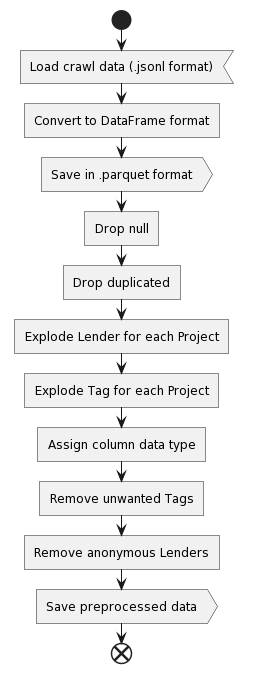
\includegraphics[width=0.2\textwidth]{images/graphuml/preprocessing.png}
	\caption{Preprocessing steps}
	\label{fig:preprocessing}
\end{figure}

Figure \ref{fig:preprocessing} shows the steps of preprocessing.
We will explains each step in detail in the following sections.
But before it, we would like to list the tools that we use for the task.
We use Python as the language of choice.
When it comes to process data in Python, perhap the most popular library is \textit{pandas}\cite{pandas}.
We took a step further and use \textit{cuDF}\cite{cudf} library, which is a GPU-accelerated version of pandas.
The reason for that is because we would like to have a fast processing time.
So we can quickly iterate over the preprocessing steps.
Meaning that we can try many different preprocessing steps and choose the one most suitable for our analysis.
We also use \textit{Dask}\cite{dask} library to handle bigger-than-memory data.
This is because at first, we do not came up with a good preprocessing pipeline.
We could easily have to process the amount of data that is too large for a GPU to handle.
We use Dask to use multiple GPUs to be able to process the whole dataset.
Although we do not use Dask in the final pipeline, we still cite it here because it is a very useful tool.
In the future works, when the data is even larger than in this thesis, one might found it helpful to use Dask.

The preprocessing pipeline begin with loading the crawled data.
Because the preprocessing steps are not appearantly clear.
We need to explore the data to find out what are the problems.
Hence, it is always a good practice to be able to load the crawled data quickly.
The first things, we use pandas to load the whole crawled data (in \lstinline|.jsonl| format) to memory.
This is possible because the raw data file is roughly 9GB, which is not too large for modern computer.
Right after that, we save the data to a \lstinline|.parquet| file for later use,
because the \lstinline|.parquet| offer much better data compression as well as faster loading time.

Next, two basic preprocessing steps that perhaps will always be done is to check for missing values and duplicated values.
In our case, the missing values and duplicated values are caused by the way that API offer data for us.
In the long duration time of crawling, it is possible that the data in the API will change.
Perhap some new Projects could be add to the platform.
But we decided that, the number of changed is not important for our analysis because the number of changed is small compared to the total number of Projects.
We remove rows that contains all null values.
Then we remove duplicated rows, consider the "id" (a.k.a "project\_id") field as the key.

Look carefully at the example row provided in \ref{tab:example-data},
we can see that each Projects could have a List of Lenders, and a List of Tags.
Fortunately, the pandas library provide a convenient way to expand those List into multiple rows.
We use the \lstinline|pandas.explode| function to do that.

Next steps, we try to assign a correct data type for each column.
In a nutshell, \lstinline|lender_id|, \lstinline|project_id| should be integer.
Some other fields should be of type \textit{category} because they have a small number of unique values.
Those fields include \lstinline|sector_name|, \lstinline|activity_name|, \lstinline|geocode_country_name|, \lstinline|tag|.
We repeat the assignment with datetime, and float types.

Next steps is to fix the Tag data.
It take us a while to understand the tags data, because some of the tags appear too frequently in the data.
Despite of that, these frequent-tags are not appear in the website interface.
We suppose that these tags are used internally by Kiva to manage the data.
We found that these tags are correspond to the \lstinline|vocabularyId = 1|,
they are \lstinline|volunteer_pick|, \lstinline|volunteer_like|, \lstinline|user_like|, \lstinline|user_favorite|.
We decide to get rid of these tags.




\section{Basic data statistics}

\begin{itemize}
	\item Worldwide statistics
	      \begin{itemize}
		      \item How many projects
		      \item how many lenders
		      \item projects vs country distribution
		      \item successful rate
		      \item \textbf{How long that users stay on the platform}
	      \end{itemize}
	\item Vietnam statistics
	      \begin{itemize}
		      \item How many projects
		      \item \dots
	      \end{itemize}
\end{itemize}
\chapter{Hypothesis testing}
\begin{itemize}
	\item The creatioon of Lender-Criteria bipartite graphs
	\item Explain why we could not project Lender-Criteria graphs onto Lender to create Lender-Lender graph
	\item That's why we find communify directly in bipartite graphs
	\item Methodology: better-than-random testing
\end{itemize}

\section{Hypothesis testing on syntehsis data}

\begin{itemize}
	\item How to build a random graph, with community pre-defined
	\item Detecting community in random graph
	\item Quality assessment of the detected community, presented by a numer $Q_{synthesis}$
	\item $Q_{synthesis}$ gives an idea about the best we could get from a data, but depends on the laten parameters when building datasets $p_{in}$, $p_{out}$, $p_{change}$ - the change from community to another
\end{itemize}

\section{Hypothesis testing on real data}

\begin{itemize}
	\item Filter data to keep Lenderes who is active invest from 2019-2023
	\item Rpeat the works on random graph for each year data
	\item Then find quality assessment $Q_{real}$ again and compare with $Q_{synthesis}$.
	      Decide if there is a clear community for different criteria (Tags, Sectors, Country)
\end{itemize}
\chapter{Conclusions and future works}
\section{Conclustions}
\begin{comment}

This community finding is a unsupervised problem.
Hence, there are different methodology for answer the question


SOmething to try

- \lstinline|adjusted_rand_score|

\section{Future works}

\begin{itemize}
	\item Extend to other platforms
	\item Transform the problem into a classical clustering problem where cluster is a Tag/Sector
	      and apply classical dynamic clustering tools.
	      Note that this part is currently in trying phase.
	      If we have time to make it now, we could move it to the section 4.
\end{itemize}
\end{comment}

In this thesis, we have studied the dynamics of crowdfunding, with a focus on the role of community.

We have first reviewed the related works on crowdfunding and on community detection problems.
We have show studies on community detection on graphs is still an active research field,
and there are many different approaches to the problem.
If focus on bipartite graphs, two main approaches are \textit{projection} and \textit{non-projection} methods.
We have observed that most of the works on community detection is a supervised problem,
while in our case, it is to apply algorithms on the unsupervised data and see if the results make sense.

We have proposed a methodology for detecting communities of lenders on crowdfunding platforms.
By devide the dataset into time slices or snapshots
and apply community detection on bipartite graphs techniques on each snapshot,
we can find groups of lenders at each snapshot.
Then we study the correlation between the groups of lenders at different snapshots,
by this way we can find groups of lenders that are stable over time and have similar lending behaviors.
If the results is better than a random baseline, we can conclude that there are communities of lenders on the platform.

We have applied this methodology to the Kiva.org platform.
First we describe the platform and how to collect data from it.
Through API, we have collected data about Lenders, Projects, Sectors, Tags, Countries.
The data alone should not be undervalued,
because through literature we do not find any other works that have collected data from Kiva.org.
With the sheer size of the data and the lack of official documentation about the data schema,
we have done heavily data explornation and preprocessing,
which could help other researchers who want to work on this dataset.

After understand those data through statistical analysis,
we built graph-like databases from the data,
and applied community detection on bipartite graphs techniques to find communities of lenders in the database.
We have found some specific groups of lenders that show repeated lending behaviors.
They are a community related to the \textit{Agriculture} sector,
or a community contribute repeatedly to the same country - Kenya.

Although the results are not very good in a sense that the methodology yields many false positives,
and the found communities might need further analysis (via sociality studies for example),
we confident that the methodology is valid and can be applied to other platforms.

In the future, several improvements can be made for the methodology.
Take building the random baseline for example,
we can relax the assumption with a larger number of lenders,
or do not assume that the groups of lenders are disjoint,
or change the number of community over time.
We can also try other methods for finding groups of people who are in same interest,
like using classical clustering algorithms with input features are Tags or Sectors or Countries or all of them.
Similarity between timestamp can also be measured in other ways, for example using Rand index.

% contribution to the OMICROWD project
This master thesis positively contributes to the OMICROWD project.
The dataset we have collected can be used as a starting point for further research on crowdfunding.
The methodology we have proposed can be applied to other platforms.
The challenges we have faced during the thesis can be used as a reference for future works.



% To better understanding the role of community in crowdfunding, we can also try to find communities of borrowers.





% appendix

\bibliographystyle{plain} % Choose a style that suits your requirements
\bibliography{kiva-writing}  % Without the .bib extension

\end{document}